\documentclass[%
    9pt,
    %handout
]{beamer}
\usepackage{graphicx} % For including single page pdfs
\usepackage{graphbox}
\usepackage{tikz}
\usepackage{layouts}


\usepackage{cambridge_lecture}
\hypersetup{colorlinks=false}



\title{Likelihood-free inference}
\subtitle{GAMBIT X}
\author[Handley] % (optional, for multiple authors)
{Will Handley\\ \small{wh260@cam.ac.uk}}
\institute[University of Cambridge] % (optional)
{%
    
\includegraphics[width=0.2\textwidth]{kicc.png}\\
    Kavli Institute for Cosmology\\
    Cavendish Laboratory (Astrophysics Group) \\
    University of Cambridge
}
\date{June 6\textsuperscript{th} 2019}

\usepackage{calculator}

\newcommand{\cols}[3][0.5]{%
    \SUBTRACT{1.}{#1}{\wdthb}
    \begin{columns}
        \begin{column}{#1\textwidth}
            #2
        \end{column}
        \begin{column}{\wdthb\textwidth}
            #3
        \end{column}
    \end{columns}
}

\newcommand{\figname}{}
\newenvironment{figright}[2][0.5]{%
    \renewcommand{\figname}{#2}
    \SUBTRACT{1.}{#1}{\wdthb}
    \begin{columns}
        \begin{column}{#1\textwidth}
        }{%
        \end{column}
        \begin{column}{\wdthb\textwidth}
            \includegraphics[width=\textwidth]{\figname}
        \end{column}
    \end{columns}
}

\newcommand{\dfigname}{}
\newenvironment{dfigright}[3][0.5]{%
    \renewcommand{\figname}{#2}
    \renewcommand{\dfigname}{#3}
    \SUBTRACT{1.}{#1}{\wdthb}
    \begin{columns}
        \begin{column}{#1\textwidth}
        }{%
        \end{column}
        \begin{column}{\wdthb\textwidth}
            \includegraphics[width=\textwidth]{\figname}
            \includegraphics[width=\textwidth]{\dfigname}
        \end{column}
    \end{columns}
}



\newenvironment{figleft}[2][0.5]{%
    \SUBTRACT{1.}{#1}{\wdthb}
    \begin{columns}
        \begin{column}{#1\textwidth}
            \includegraphics[width=\textwidth]{#2}
        \end{column}
        \begin{column}{\wdthb\textwidth}
        }{%
        \end{column}
    \end{columns}
}

\newenvironment{dfigleft}[3][0.5]{%
    \SUBTRACT{1.}{#1}{\wdthb}
    \begin{columns}
        \begin{column}{#1\textwidth}
            \includegraphics[width=\textwidth]{#2}
            \includegraphics[width=\textwidth]{#3}
        \end{column}
        \begin{column}{\wdthb\textwidth}
        }{%
        \end{column}
    \end{columns}
}


\newcounter{numimages}

\newenvironment{multifig}[1]{%
    \begin{frame}
        \pdfximage{#1}%
        \setcounter{numimages}{\the\pdflastximagepages}
        \addtocounter{numimages}{-1}

        \begin{tikzpicture}[remember picture, overlay]
            \foreach \pagenum in {1,...,\thenumimages} {%
                \node<handout:0|beamer:\pagenum>[anchor=center] at (current page.center) {
                \includegraphics[width=\textwidth,page=\pagenum]{#1}}; 
            }
            \addtocounter{numimages}{1}
            \node<handout:1|beamer:\thenumimages>[anchor=center] at (current page.center) {
            \includegraphics[width=\textwidth,page=\thenumimages]{#1}}; 
        \end{tikzpicture}
    }{%
    \end{frame}
}


\newcommand{\vect}[1]{\mathbf{#1}}
\newcommand{\bg}[1]{\mathbf{#1}}
\newcommand{\red}[1]{\textcolor{cambblue}{#1}}
\newcommand{\blue}[1]{\textcolor{red}{#1}}
\newcommand{\black}[1]{\textcolor{black}{#1}}
\newcommand{\rr}{\Rightarrow}
\newcommand{\arxiv}[1]{\href{https://arxiv.org/abs/#1}{arXiv:#1}}

\begin{document}

\begin{frame}
    \titlepage{}
\end{frame}

\begin{frame}
    \frametitle{Likelihood free inference: what's in a name?}
    \begin{itemize}
        \item The term ``Likelihood-free'' is a misnomer -- there is still very much a likelihood involved in the analysis
        \item LFI is a framework for situations where you don't know what the likelihood is, but can still simulate your system
            \begin{itemize}
                \item i.e.\ you are freed from having to write down the likelihood explicitly
            \end{itemize}
        \item Fundamental idea: construct a flexible proxy likelihood, and fit this to simulations.
        \item Fitted likelihood can then be used in both Frequentist and Bayesian analyses.
        \item Related to Approximate Bayesian Computation (ABC) but better.
        \item Key references from cosmology:
            \begin{itemize}
                \item \arxiv{1801.01497}
                \item \arxiv{1903.00007}
                \item \arxiv{1903.01473}
                \item \arxiv{1904.05364}
                \item Another paper coming soon: ``Compromise-free Likelihood-free inference''
            \end{itemize}
    \end{itemize}
\end{frame}

\begin{frame}
  \frametitle{Motivating example: Cosmological large-scale structure}
  \begin{figleft}[0.7]{./figures/dm.jpeg}
      \begin{itemize}
          \item What is the likelihood $P(D|\theta)$ for large scale structure formation?
          \item Can simulate data $\hat{D}$ given set of cosmological parameters $\theta$.
          \item Image shows effect of varying the amount of dark matter in simulation
          \item Would like to compare simulation to actual data: $\chi^2(\theta) \sim |\hat{D}(\theta) - D |^2$
      \end{itemize}
  \end{figleft}
\end{frame}

\begin{frame}
  \frametitle{Two key problems}
  \[\chi^2(\theta) \sim |\hat{D}(\theta) - D |^2\]
  \begin{enumerate}
      \item Datasets are in general exponentially large
          \begin{itemize}
              \item The whole point of science is to compress data into models with a small number of parameters.
          \end{itemize}
      \item What is the correct metric to measure the difference between $\hat{D}$ and $D$?
          \begin{itemize}
              \item ABC works by rejection sampling up to some $\epsilon$ difference above to select the correct $\theta$.
          \end{itemize}
  \end{enumerate}
  The recent advance in LFI is a framework that solves both of these problems.
\end{frame}

\begin{frame}
  \frametitle{Solution 1: Massive compression}
      \begin{itemize}
          \item All we are interested in is ``What do the data $D$ tell me about the $n$ parameters of my model $\theta$?''
          \item In theory, the dataset $D$ should be compressible into $n$ numbers without losing information about $\theta$.
          \item For example, when inferring the underlying mean $\mu$ and variance $\sigma^2$ of some numbers $\{x_1,\cdots,x_d\}$, all you need is the sample mean $\bar{x}$ and sample variance $S^2$ (c.f.\ sufficient statistics).
      \end{itemize}
      {\Large
      $\theta = [\Omega_m, \Omega_b, \sigma_8]$
      \hfill
      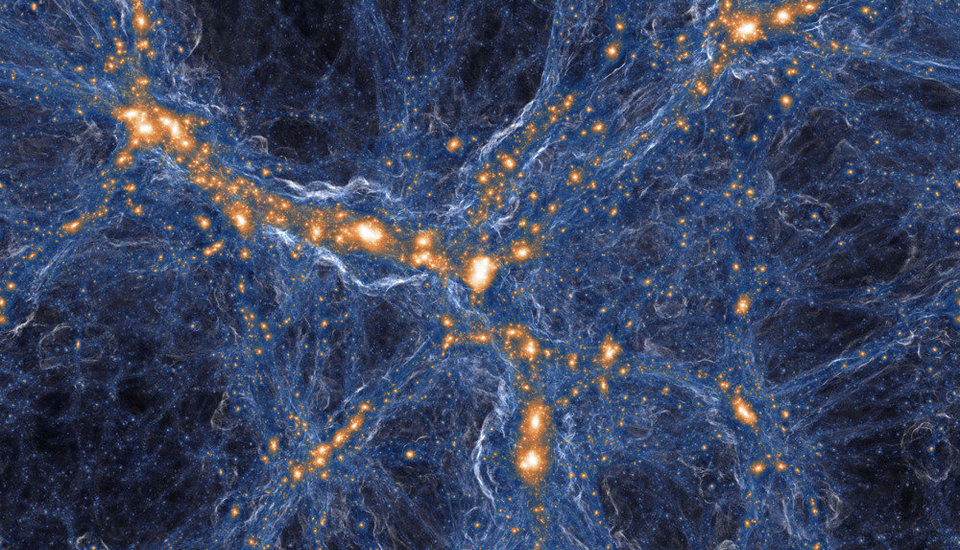
\includegraphics[align=c,width=0.4\textwidth]{./figures/simulation.jpg}
      \hfill
      $\longrightarrow  D=[0.3, 0.4, 0.9]$
      }
      \begin{itemize}
          \item The advance in cosmology which made the recent work possible (\arxiv{1712.00012}) was to generalise Karhunen-Lo\'{e}ve  and MOPED to {\em score  compression}:
              \begin{itemize}
                  \item If you have an approximate likelihood $L(\theta)$, then $\nabla_\theta L$ is in some sense an optimal compression.
              \end{itemize}
          \item More compression schemes are possible: watch this space.
      \end{itemize}
\end{frame}

\begin{frame}
  \frametitle{Solution 2: Density estimation}
      \begin{itemize}
          \item One can generate a set of $K\sim1000$ training simulations $\{(D_1,\theta_1),\cdots,(D_K,\theta_K)\}$.
          \item Apply compression, and these are samples in a $2n$-dimensional space.
          \item Build a proxy joint distribution $P(\theta,D) = f(\theta, D; \alpha)$ with some free parameters $\alpha$:
          \item With this proxy joint, one has a likelihood of $\alpha$ defined by:
              \[
                  L(\alpha) = \prod_{i=1}^K f(\theta_i, D_i; \alpha)
              \]
          \item Use $L(\alpha)$ as a misfit function for maximising/marginalising $\alpha$.
      \end{itemize}
      \begin{columns}
        \begin{column}{0.4\textwidth}
              \begin{itemize}
                  \item Gaussian mixture models
                  \item Neural density estimators
                  \item \ldots
              \end{itemize}
        \end{column}
        \begin{column}{0.6\textwidth}
            \hfill
            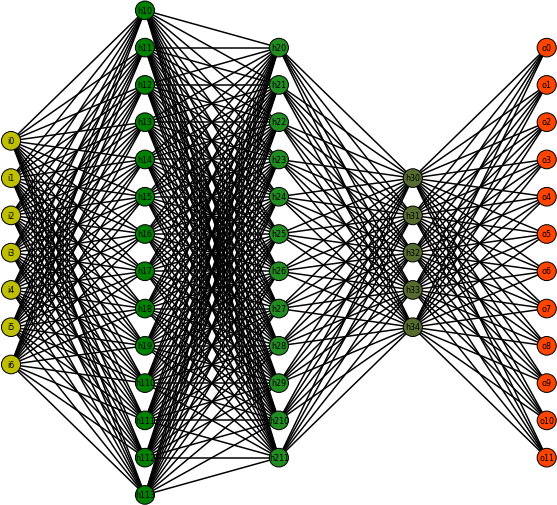
\includegraphics[width=0.35\textwidth]{./figures/nn.png}
            \hfill
            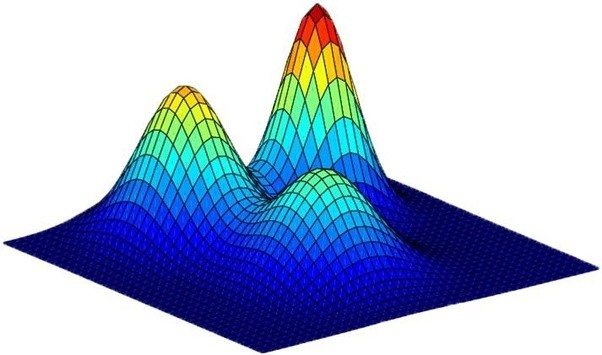
\includegraphics[width=0.6\textwidth]{./figures/mixture_gaussian.jpeg}
            \hfill
        \end{column}
      \end{columns}
\end{frame}

\begin{frame}
    \frametitle{The full framework}
    \begin{enumerate}
        \item In lieu of a likelihood, write data simulator $\hat{D}(\theta)$
        \item Generate training data $\{(D_1,\theta_1),\cdots,(D_K,\theta_K)\}$
        \item Choose massive compression scheme (e.g. score) and compress training data
        \item Choose proxy distribution $f(D, \theta; \alpha)$ (e.g. neural density estimator) and fit to training data to give e.g. $P(D,\theta) = f(D, \theta; \alpha_\mathrm{max})$
        \item Use trained joint for all your usual inference:
            \begin{itemize}
                \item Can calculate likelihood by inputting the actual data (in compressed form)
                \item For some proxy distributions (e.g. mixture models) you can get the evidence for free.
            \end{itemize}
    \end{enumerate}
\end{frame}

\begin{frame}
    \frametitle{Cosmological examples}
    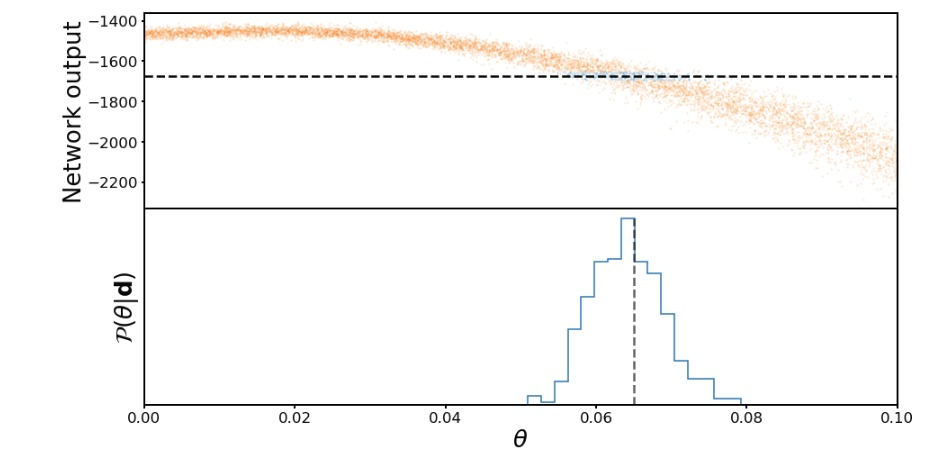
\includegraphics[width=0.59\textwidth]{./figures/tau.jpeg}
    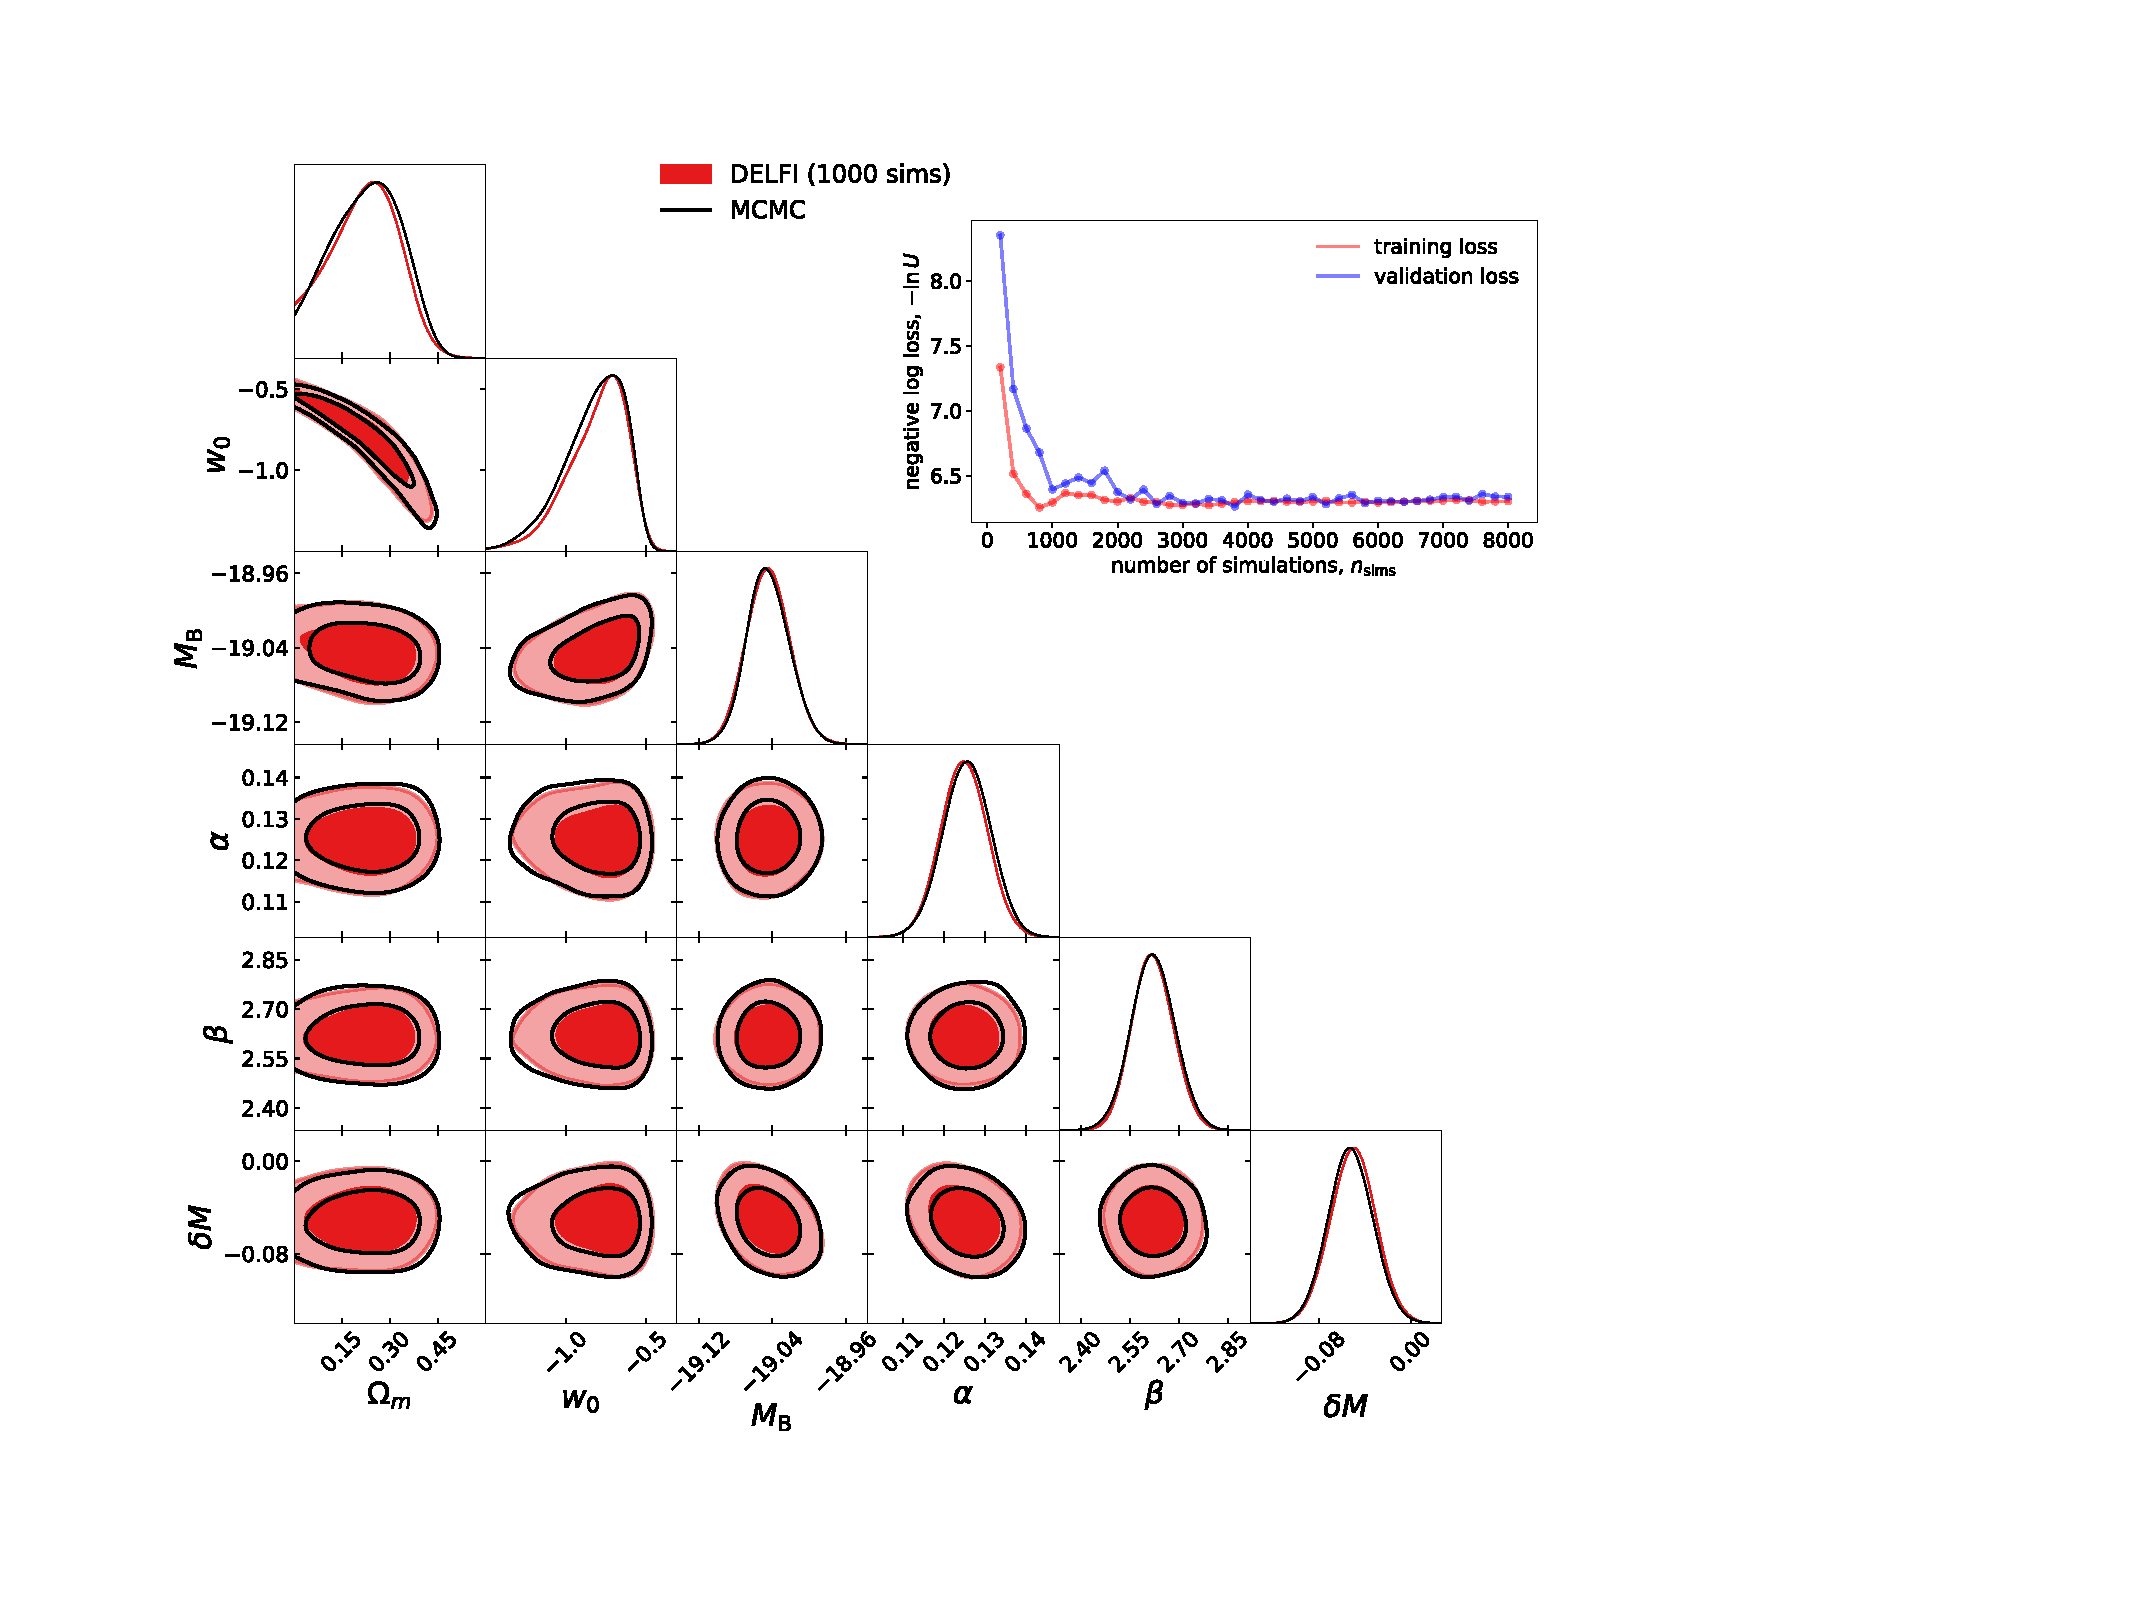
\includegraphics[width=0.39\textwidth]{./figures/jla_contours_insert.pdf}
    My research:
    \begin{itemize}
        \item Instead of maximising wrt $\alpha$, in a Bayesian framework one should marginalise
        \item Can use Bayesian evidences to select the best proxy, and to pick/marginalise over the number of mixture components/neural network nodes.
    \end{itemize}
\end{frame}

\begin{frame}
    \frametitle{Summary}
    \begin{itemize}
        \item Recent advances have brought LFI into the realm of ``possible'' with current technology
        \item In ten years time, with advances in both theory and computing power everyone will be doing this (think MCMC twenty years ago).
        \item GAMBIT should be thinking about incorporating these techniques over the next few years.
    \end{itemize}
\end{frame}

\end{document}
